\documentclass[pdftex]{beamer}  % For use with beamer v 2.20  
\mode<presentation>

%\usepackage[utf8]{inputenc}
%\usepackage[english,hebrew]{babel}

\usepackage{multimedia}
\usepackage{xcolor}
\usepackage{tikz}
\usepackage{tikzit}
%\input{sample.tikzstyles}
\usepackage{graphicx}
\usepackage{wasysym}
\usepackage{tikz}
\usepackage{tkz-euclide}
\usepackage{tikz}
\usetikzlibrary{shapes.geometric, arrows}


 
\usetheme{Madrid}  % JuanLesPins  Rochester  
		  
%\useinnertheme{rounded}
%\usecolortheme{crane}
%\usefonttheme{structuresmallcapsserif}

\usepackage{amsmath,amssymb}
\usepackage{graphicx,color}

\newtheorem{conjecture}[theorem]{Conjecture}


%%%%%%%%%%%%%%%%%%%%%%%%%%%%%%
\newcommand{\beql}[1]{\begin{equation}\label{#1}}
\newcommand{\eeq}{\end{equation}}
\newcommand{\comment}[1]{}
\newcommand{\Ds}{\displaystyle}
\newcommand{\Fpart}[1]{{\left\{{#1}\right\}}}
\newcommand{\Abs}[1]{{\left|{#1}\right|}}
\newcommand{\Lone}[1]{{\left\|{#1}\right\|_{L^1}}}
\newcommand{\Linf}[1]{{\left\|{#1}\right\|_\infty}}
\newcommand{\Norm}[1]{{\left\|{#1}\right\|}}
\newcommand{\Mean}{{\bf E}}
\newcommand{\Floor}[1]{{\left\lfloor{#1}\right\rfloor}}
\newcommand{\Ceil}[1]{{\left\lceil{#1}\right\rceil}}
\newcommand{\Qed}{\ \\\mbox{$\Box$}}
%\newcommand{\Qed}{\ \\\mbox{$\blacksquare$}}
\newcommand{\N}{{\bf N}}
\newcommand{\Prob}[1]{{{\bf{Pr}}\left[{#1}\right]}}
\newcommand{\Set}[1]{{\left\{{#1}\right\}}}
\newcommand{\given}{{\ |\ }}
\newcommand{\as}{{a.s.}}
\newcommand{\ToAppear}[1]{\raisebox{15mm}[10pt][0mm]{\makebox[0mm]%
   {\makebox[\textwidth][r]{\small #1}}}}
\newcommand{\siirv}{{SIIRV}}
\newcommand{\PP}{{\mathbb P}}
\newcommand{\RR}{{\mathbb R}}
\newcommand{\CC}{{\mathbb C}}
\newcommand{\ZZ}{{\mathbb Z}}
\newcommand{\NN}{{\mathbb N}}
\newcommand{\TT}{{\mathbb T}}
\newcommand{\QQ}{{\mathbb Q}}
\newcommand{\One}[1]{{\bf 1}\left(#1\right)}
\newcommand{\one}{{\bf 1}}
\newcommand{\zero}{{\bf 0}}
\newcommand{\BAR}[1]{\overline{#1}}
\newcommand{\inner}[2]{{\langle #1, #2 \rangle}}
\newcommand{\Inner}[2]{{\left\langle #1, #2 \right\rangle}}
\newcommand{\avg}{{\rm Avg\,}}
\newcommand{\dens}{{\rm dens\,}}
\newcommand{\Span}{{\rm span}}
\newcommand{\vol}{{\rm vol\,}}
\newcommand{\ft}[1]{\widehat{#1}}
\newcommand{\FT}[1]{\left(#1\right)^\wedge}
\newcommand{\nozero}[1]{{#1\setminus\Set{0}}}
\newcommand{\supp}{{\rm supp\,}}
\newcommand{\Li}{{\rm Li\,}}
\newcommand{\pp}[1]{{\left({#1}\right)}}
\renewcommand{\vec}[1]{{\mbox{\boldmath$#1$}}}
\newcommand{\pty}{\mathbf {\oplus}}
\newcommand{\ptyc}{\bf \overline{\oplus}}
\newcommand{\eat}[1]{}
\newcommand{\myframetitle}[1]{\frametitle{#1}}
% remarks on the margins
\newcounter{rem}
\setcounter{rem}{0}
\newcommand{\rem}[1]{
    \marginpar{\refstepcounter{rem}{\tiny\therem: #1}}
}



% other people's theorems
\newcounter{othm}
\setcounter{othm}{0}
\def\theothm{\Alph{othm}} 
\newenvironment{othm}{
  \sf
  \vskip 0.10in
  \refstepcounter{othm}
  \noindent{\bf Theorem\ \theothm}
}{\vskip 0.10in}


\title{$L^1$-minimization and signal recovery }  

\author[Alex Iosevich]{Alex Iosevich} 
\institute[University of Rochester ]{} 

\date{Simple ideas of great mathematicians series} 

\begin{document}

\frame{\titlepage} 

%\frame{\myframetitle{Motivation... } 
%\begin{itemize} 

%\item<+-| alert@+>   \begin{figure}
%\centering
%\includegraphics[scale=.5]{useful.jpg}
%\end{figure}


%\end{itemize} 

%} 

\frame{\myframetitle{U.S. Inflation Rate} 
\begin{itemize} 

\item<+-| alert@+>  \begin{figure}
\centering
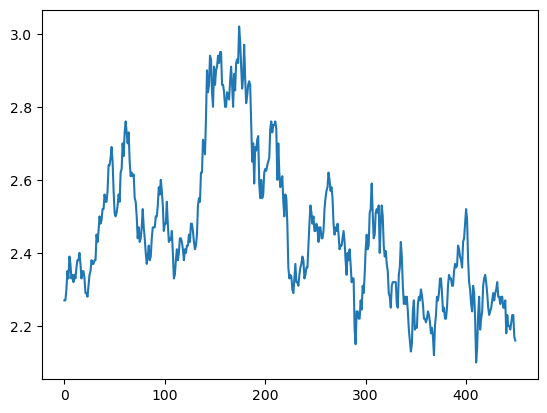
\includegraphics[scale=.6]{inflationNW.png}
\end{figure}

\end{itemize} 

} 



\frame{\myframetitle{Classical imputation using trig polynomial regression} 
\begin{itemize} 

\item<+-| alert@+> In the picture below, 150 of the 450 points in the original inflation data set are randomly removed. The values are then filled in using the trig polynomial regression. What you see is the graph of the original missing points (red) and the imputed values (black). 

\vskip.125in 

\item<+-| alert@+>  \begin{figure}
\centering
\includegraphics[scale=.45]{trigimputeNW.png}
\end{figure}

\end{itemize} 

} 

\frame{\myframetitle{Imputation using the methods of exact signal recovery} 
\begin{itemize} 

\item<+-| alert@+>  This time, the original missing values are in {\color{red} red}, the trig imputation is in {\bf black} and the method arising from the world of {\bf exact signal recovery} is in {\color{blue} blue}. 

\vskip.125in 

\item<+-| alert@+>  \begin{figure}
\centering
\includegraphics[scale=.45]{L1optimizerNW.png}
\end{figure}

\end{itemize} 

} 

\frame{\myframetitle{The purpose of this talk} 
\begin{itemize} 

\item<+-| alert@+> The purpose of this talk is to explain how some ideas from discrete Fourier analysis can be used to build and justify the  {\color{blue} "blue"} imputation mechanism above. 

\vskip.25in 

\item<+-| alert@+>  \begin{figure}
\centering
\includegraphics[scale=.6]{investopedia.jpg}
\end{figure}


\end{itemize} 

} 




\frame{\myframetitle{Finite Signals and Discrete Fourier transform} 
\begin{itemize} 
 
\item<+-| alert@+> Let $f$ be a signal of finite length, i.e $ f: {\mathbb Z}^d_N \to {\mathbb C}$. 

\vskip.25in 

\item<+-| alert@+> Suppose that  the Fourier transform of $f$ is transmitted, where 

$$ \widehat{f}(m)=N^{-\frac{d}{2}} \sum_{x \in {\mathbb Z}_N^d} \chi(-x \cdot m) f(x); \ \chi(t)=e^{\frac{2 \pi i t}{N}}.$$

\vskip.25in 

\item<+-| alert@+> Fourier Inversion says that we can recover the signal by writing 

$$ f(x)=N^{-\frac{d}{2}} \sum_{m \in {\mathbb Z}_N^d} \chi(x \cdot m) \widehat{f}(m).$$  

\end{itemize} 

} 

\frame{\myframetitle{Exact recovery problem} 
\begin{itemize} 

\item<+-| alert@+>  The basic question is, can we recover $f$ {\bf exactly} from its discrete Fourier transforms if 

$$ \left\{\widehat{f}(m): m \in S \right\}$$ are  unobserved (or missing  due to noise, other interference, or security), for some $S \subset {\mathbb Z}_N^d$? 

\vskip.25in 

\item<+-| alert@+> The answer turns out to be \boxed{YES} (Matolcsi-Szucks 1973, Donoho-Stark 1989)  if $f$ is supported in $E \subset {\mathbb Z}_N^d$, and 
$$ |E| \cdot |S|<\frac{N^d}{2},$$ with the main tool being the Fourier Uncertainty Principle. 

\end{itemize} 

} 

 
%\frame{\myframetitle{Fourier Inversion and Plancherel} 
%\begin{itemize} 

%\item<+-| alert@+> Given $f: {\mathbb Z}_N^d \to {\mathbb C}$, we shall use the following two formulas repeatedly: 


%\vskip.25in 

%\item<+-| alert@+> (Fourier Inversion) $$ f(x)=N^{-\frac{d}{2}} \sum_{m \in {\mathbb Z}_N^d} \chi(x \cdot m) \widehat{f}(m),$$ and 

%\vskip.25in 

%\item<+-| alert@+> (Plancherel) $$ \sum_{m \in {\mathbb Z}_N^d} {|\widehat{f}(m)|}^2 = \sum_{x \in {\mathbb Z}_N^d} {|f(x)|}^2.$$ 

%\end{itemize} 

%} 

 
\frame{\myframetitle{Matolcsi-Szucks/ Donoho-Stark results} 
\begin{itemize} 

\item<+-| alert@+> Suppose that $f: {\mathbb Z}^d_N \to {\mathbb C}$ is supported in $E \subset {\mathbb Z}^d_N$, with the frequencies in $S \subset {\mathbb Z}^d_N$ unobserved. 

\vskip.5in 

\item<+-| alert@+> If $f$ cannot be recovered uniquely, then there exists a signal $g: {\mathbb Z}^d_N \to {\mathbb C}$ such that $g$ also has $|E|$ non-zero entries, 
$$\widehat{f}(m)=\widehat{g}(m) \ \text{for} \ m \notin S,$$ and $f$ is not identically equal to $g$. 

 \end{itemize} 

} 

%\frame{\myframetitle{David Donoho} 
%\begin{itemize} 

%\item<+-| alert@+> David Donoho (1991 MacArthur Fellow) is one of the leading experts in the development of effective methods for the construction of low-dimensional representations for high-dimensional data problems, development of wavelets for denoising and compressed sensing.

%\vskip.25in 

%\item<+-| alert@+>  \begin{figure}
%\centering
%\includegraphics[scale=.5]{donoho.jpg}
%\end{figure}

%\end{itemize} 

%} 

\frame{\myframetitle{Uncertainty Principle $\to$ Unique Recovery} 
\begin{itemize} 

\item<+-| alert@+> Let $h=f-g$. It is clear that $\widehat{h}$ has at most $|S|$ non-zero entries, and $h$ has at most $2|E|$ non-zero entries. 

\vskip.25in 

\item<+-| alert@+> By the Fourier Uncertainty Principle, 
$$ 2|E| \cdot |S| \ge N^d.$$  

\vskip.25in 

\item<+-| alert@+> It would then follow that if we assume 
$$ |E| \cdot |S| < \frac{N^d}{2},$$ we must have $h=0$, and hence  the recovery is {\it unique}.  

\end{itemize} 

} 

\frame{\myframetitle{$L^1$ minimization algorithm} 
\begin{itemize} 

\item<+-| alert@+> Donoho and Stark showed, using a beautiful idea due to Benjamin Logan, that if $f: {\mathbb Z}_N^d \to {\mathbb C}$ is supported in $E$, and the frequencies ${\{\widehat{f}(m)\}}_{m \in S}$ are unobserved, then if 
$$ |E| \cdot |S|<\frac{N^d}{2},$$ 

\vskip.25in 

\item<+-| alert@+> then $f$ can be recovered as 
$$ arg \ min_{u} \ {||u||}_{L^1({\mathbb Z}_N^d)} \ \text{subject to} \ \widehat{f}(m)=\widehat{u}(m) \ \text{for} \ m \notin S.$$ 

\end{itemize} 

} 

\frame{\myframetitle{Benjamin Franklin Logan (1927-2015)} 
\begin{itemize} 

\item<+-| alert@+> Logan was an accomplished bluegrass musician in addition to his groundbreaking scientific work . His most famous publication is the song, entitled "Christmas Time is Coming", performed by Johnny Cash and many others. 

\vskip.25in 

\begin{figure}
\centering
\includegraphics[scale=.6]{logan.jpg}
\end{figure}

\end{itemize} 

} 


%\begin{frame}{Christmas Time is Coming}
%\begin{figure}
%\centering
%\includegraphics[scale=.2]{ChristmasTime.png}
%\end{figure}

%\href{https://www.youtube.com/watch?v=3CUB4aJ07cE}{Here is (by far) the most famous publication of Benjamin Franklin Logan!}
%\end{frame}


\frame{\myframetitle{Proof of the $L^1$ recovery method} 
\begin{itemize} 

\item<+-| alert@+> Let $f=g+h$, where $g$ is the solution to the $L^1$ minimization problem above, and note that $\widehat{h}$ is supported in $S$. We have 
$$ {||g||}_{L^1({\mathbb Z}_N^d)}= {||f-h||}_{L^1({\mathbb Z}_N^d)}$$
 $$={||f-h||}_{L^1(E)}+{||h||}_{L^1(E^c)} \ge {||f||}_{L^1({\mathbb Z}_N^d)}+\left[ {||h||}_{L^1(E^c)} -{||h||}_{L^1(E)} \right].$$
 
 \vskip.125in 

\item<+-| alert@+> If we can show that ${||h||}_{L^1(E^c)}>{||h||}_{L^1(E)}$, then $${||f||}_{L^1({\mathbb Z}_N^d)}<{||g||}_{L^1({\mathbb Z}_N^d)},$$ which is impossible since $g$ is the $L^1$ minimizer. 

\vskip.125in 

\item<+-| alert@+> The resulting contradiction will prove that $h \equiv 0$. 

\end{itemize} 

} 

%\frame{\myframetitle{The uncertainty principle strikes again} 
%\begin{itemize} 

%\item<+-| alert@+> We have 
%$$ |h(x)| = N^{-\frac{d}{2}} \cdot \left| \sum_{m \in S} \chi(x \cdot m) \widehat{h}(m) \right| \leq N^{-d}  \cdot |S| \cdot {||h||}_{L^1({\mathbb Z}_N^d)}.$$ 

%\vskip.25in 

%\item<+-| alert@+> It follows that 
%$$ {||h||}_{L^1(E)} \leq N^{-d} \cdot |E| \cdot |S| \cdot {||h||}_{L^1({\mathbb Z}_N^d)}<\frac{1}{2} \cdot {||h||}_{L^1({\mathbb Z}_N^d)}.$$ 

%\vskip.25in 

%We conclude that 
%$$ {||h||}_{L^1(E)}<{||h||}_{L^1(E^c)},$$ as desired. 

%\end{itemize} 

%} 

\frame{\myframetitle{Can we loosen the $|E| \cdot |S|<\frac{N^d}{2}$ assumption?} 
\begin{itemize} 

\item<+-| alert@+> In general, the answer is no. Suppose that $d=1$, $N$ {\bf is not} prime, and $E$ is a subgroup of ${\mathbb Z}_N$.

\vskip.25in 

\item<+-| alert@+> Then if $f$ is supported on $E$, $\widehat{f}$ is supported on the annihilator subgroup 
$$ S=\{m \in {\mathbb Z}_N: xm=0 \ \forall \ x \in E \}.$$

\vskip.25in 

\item<+-| alert@+> Since $|E| \cdot |S|=N$, we see that the Donoho-Stark recovery condition cannot be improved, up to a constant, since $S$ can be a set of missing frequencies. 

\vskip.25in 

\item<+-| alert@+> However, we shall that for a generic set $S$ of missing frequencies, the situation is much better. 

\end{itemize} 

} 

%\frame{\myframetitle{The prime case $d \ge 2$} 
%\begin{itemize} 

%\item<+-| alert@+> If $N$ is prime and $d \ge 2$, it is not difficult to check that if $f$ is supported on a $k$-dimension plane $H$, $\widehat{f}$ is supported on the orthogonal subspace $H^{\perp}$. 

%\vskip.25in 

%\item<+-| alert@+> It follows that the classical uncertainty principle is sharp in this case, and the Donoho-Stark recovery condition cannot be improved, up to a constant. 

%\vskip.25in 

%\item<+-| alert@+> \begin{figure}
%\centering
%\includegraphics[scale=.5]{orthogonalsubspace.png}
%\end{figure}

%\end{itemize} 

%} 

%\frame{\myframetitle{The prime case $d=1$} 
%\begin{itemize} 

%\item<+-| alert@+> If $N$ is prime and $d=1$, a beautiful result due to Terry Tao says that if $f$ is supported on $E$ and $\widehat{f}$ is supported on $S$, then 
%$$|E|+|S| \ge N+1, $$ with the corresponding improvement for the exact signal recovery condition. 

%\vskip.25in 

%\item<+-| alert@+> This result is a consequence of a beautiful 1924 result due to Chebotaryov, which says that every $k$ by $k$ minor of the Fourier matrix 
%$${\left\{e^{-\frac{2 \pi i xm}{N}} \right\}}_{x \in {\mathbb Z}_N, m \in {\mathbb Z}_N} $$ is non-singular if $N$ is an odd prime. 

%\end{itemize} 

%} 

\frame{\myframetitle{Bourgain's $\Lambda_q$ theorem - general formulation} 
\begin{itemize} 

\item<+-| alert@+> Jean Bourgain (1989) proved that if $G$ is a locally compact abelian group, $\phi_1, \dots, \phi_n$ are orthogonal functions with 
${||\phi_j||}_{\infty} \leq 1$, the for a generic set $S \subset \{1,2, \dots, n\}$ of size $\lceil n^{\frac{2}{q}} \rceil$, $q>2$, 

$$ {\left|\left| \sum_{i \in S} a_i \phi_i \right|\right|}_{L^q(G)} \leq C(q) \cdot {\left( \sum_{i \in S} {|a_i|}^2 \right)}^{\frac{1}{2}},$$ where $C(q)$ depends only on $q$. 

\vskip.25in 

\item<+-| alert@+>  As we shall see, this result has a simple and effective built-in uncertainty principle. 

\end{itemize} 

} 

%\frame{\myframetitle{Jean Bourgain} 
%\begin{itemize} 

%\item<+-| alert@+> Jean Bourgain (Fields Medal 1994) has done groundbreaking work in a variety of areas of mathematics, weaving together techniques from analysis, probability, combinatorics and number theory. Reading his papers is an incredibly rewarding, if somewhat painful, process. 

%\vskip.25in 

%\begin{figure}
%\centering
%\includegraphics[scale=.5]{bourgain.jpg}
%\end{figure}

%\end{itemize} 

%} 

\frame{\myframetitle{Bourgain's $\Lambda_q$ theorem} 
\begin{itemize} 

\item<+-| alert@+> It is a consequence of Bourgain's celebrated $\Lambda_p$ theorem in locally compact abelian groups that if $f: {\mathbb Z}_N^d \to {\mathbb C}$ and {\bf $\widehat{f}$ is supported in $S$}, then for a "generic" set of size $\lceil N^{\frac{2d}{q}} \rceil$, $2<q<\infty$, 
$$ {\left( \frac{1}{N^d} \sum_{x \in {\mathbb Z}_N^d} {|f(x)|}^{q} \right)}^{\frac{1}{q}} \leq C(q) {\left( \frac{1}{N^d} \sum_{x \in {\mathbb Z}_N^d} {|f(x)|}^2 \right)}^{\frac{1}{2}},$$ with $C(q)$ independent of $N$. 

\vskip.25in 

\item<+-| alert@+> It is not difficult to see that this inequality implies that the support of $f$ must be a positive proportion of ${\mathbb Z}_N^d$. 

\end{itemize} 

} 

\frame{\myframetitle{Signal recovery in the presence of the $\Lambda_q$ inequality} 
\begin{itemize} 

\item<+-| alert@+> \begin{theorem} (A. Iosevich and A. Mayeli (ACHA 2024)) Let $f: {\mathbb Z}_N^d \to {\mathbb C}$ be a signal supported in $E \subset {\mathbb Z}_N^d$. Suppose that the frequencies ${\{\widehat{f}(m)\}}_{m \in S}$ are unobserved, where $S$ satisfies the $\Lambda_q$ inequality with constant $C(q)$, i.e whenever $\widehat{g}$ is supported in $S$, $|S|=\lceil N^{\frac{2d}{q}} \rceil$, 
$$ {\left( \frac{1}{N^d} \sum_{x \in {\mathbb Z}_N^d} {|g(x)|}^{q} \right)}^{\frac{1}{q}} \leq C(q) {\left( \frac{1}{N^d} \sum_{x \in {\mathbb Z}_N^d} {|g(x)|}^2 \right)}^{\frac{1}{2}},$$ with $C(q)$ independent of $N$. Then $f$ can be recovered exactly and uniquely provided that 
$$ |E|< \frac{N^d}{2{(C(q))}^{\frac{1}{\frac{1}{2}-\frac{1}{q}}}},$$ 

\end{theorem} 

\end{itemize} 

} 

\frame{\myframetitle{A direct consequence of Bourgain's $\Lambda_q$ theorem} 
\begin{itemize} 

\item<+-| alert@+> Suppose that $S$ is generic, as in Bourgain's theorem. 

\vskip.25in 

\item<+-| alert@+> Suppose that $f$ is supported in $E \subset {\mathbb Z}_N^d$ and $\widehat{f}$ is supported in $S$. Bourgain's theorem implies that 

\vskip.25in 

\item<+-| alert@+> $$ N^{-\frac{d}{q}} \cdot {|E|}^{\frac{1}{q}} {\left( \frac{1}{|E|} \sum_{x \in E} {|f(x)|}^{q} \right)}^{\frac{1}{q}}$$
$$ \leq C(q) N^{-\frac{d}{2}} \cdot {|E|}^{\frac{1}{2}} {\left( \frac{1}{|E|} \sum_{x \in E} {|f(x)|}^2 \right)}^{\frac{1}{2}}.$$

\end{itemize} 

} 

\frame{\myframetitle{A direct consequence of Bourgain's $\Lambda_q$ theorem} 
\begin{itemize} 

\item<+-| alert@+> It follows that 
$$ |E| \ge \frac{N^d}{{(C(q))}^{\frac{1}{\frac{1}{2}-\frac{1}{q}}}}.$$ 

\vskip.25in 


\item<+-| alert@+> We conclude that if we send the Fourier transform of a signal $f$ supported on a set of size 
$$<\frac{N^d}{2{(C(q))}^{\frac{1}{\frac{1}{2}-\frac{1}{q}}}},$$ and the frequencies in $S \subset {\mathbb Z}_N^d$, $|S|=\lceil N^{\frac{2d}{q}} \rceil$, satisfying the $\Lambda_q$, $q>2$, inequality with constant $C(q)$ are missing, we can recover $f$ exactly with very high probability using the rather inefficient method of least squares. 

\end{itemize} 

} 

\frame{\myframetitle{Talagrand's theorem (general)} 
\begin{itemize} 

\item<+-| alert@+> The general form of Talagrand's theorem (the first result of this type following Bourgain's 1989 result) is the following. 

\vskip.125in 

\item<+-| alert@+> \begin{theorem} (Talagrand 1998) Let ${\{\phi_j\}}_{j=1}^n$ be an orthonormal system in $L^2$ with $|\phi_j(x)| \leq 1$, $1 \leq j \leq n$. There exists a constant $\gamma_0 \in (0,1)$ and a generic subset $S \subset \{1, \dots, n\} $ with $ |S| \leq \gamma_0 n $ such that for every $a = (a_i) \in \mathbb{C}^n$,

$$ \left( \sum_{i \in S} {|a_i|}^2 \right)^{\frac{1}{2}} \leq C_T \sqrt{\log(n) \log \log(n)} \cdot {\left| \left| \sum_{i \in I} a_i \phi_i \right| \right|}_{L^1}.$$ 

where $C_T > 0$ is a universal constant.
\end{theorem} 

\end{itemize} 

} 

\frame{\myframetitle{Talagrand's theorem in our context} 
\begin{itemize} 

\item<+-| alert@+> In the context of functions mapping ${\mathbb Z}_N^d \to {\mathbb C}$, Talagrand's theorem takes on the following form. 

\vskip.125in 

\item<+-| alert@+> \begin{theorem} There exists $\gamma_0 \in (0,1)$ such that if $h: {\mathbb Z}_N^d \to {\mathbb C}$ with $\widehat{h}$ supported in a generic set $S$ of size $|S| \leq \gamma_0 \frac{N^d}{\log(N)}$, then with probability $1-o_N(1)$, 
$$ {\left( \frac{1}{N^d} \sum_{x \in {\mathbb Z}_N^d} {|h(x)|}^2 \right)}^{\frac{1}{2}} \leq C_T \sqrt{\log(N^d) \log \log(N^d)} \cdot \frac{1}{N^d} \sum_{x \in {\mathbb Z}_N^d} |h(x)|.$$
\end{theorem} 

\end{itemize} 

} 

%\frame{\myframetitle{Michel Talagrand} 
%\begin{itemize} 

%\item<+-| alert@+> Michel Talagrand (Abel Prize 2024) is one the greatest living experts on probability and functional analysis. 

%\vskip.25in 

%\item<+-| alert@+> \begin{figure}
%\centering
%\includegraphics[scale=.5]{talagrand.jpg}
%\end{figure}

%\end{itemize} 

%} 

\frame{\myframetitle{A slight variant of a result due to Iosevich, Kashin, Limonova, and Mayeli (2024)} 
\begin{itemize} 

\item<+-| alert@+> \begin{theorem} There exists $\gamma_0 \in (0,1)$ such that if $f: {\mathbb Z}_N^d \to {\mathbb C}$ with ${\{\widehat{f}(m)\}}_{m \in S}$ unobserved, where $S$ is a generic set of size $ \leq \gamma_0 N^d$, then if 
$$ |\{x \in {\mathbb Z}_N^d: f(x) \not=0 \}| \leq \frac{1}{4C_T} \frac{N^d}{\log(N^d) \log \log(N^d)},$$ then $f$ can be recovered uniquely using the algorithm 
$$ g = arg min_u {||u||}_1 \ \text{with the constraint} \ \widehat{u}(m)=\widehat{f}(m) \ \text{for} \ m \notin S.$$ 

\end{theorem} 

\end{itemize} 

} 

%\frame{\myframetitle{Sketch of proof of the Iosevich, Kashin, Limonova, and Mayeli (2024)} 
%\begin{itemize} 

%\item<+-| alert@+> As always, we write $f=g+h$, where $\widehat{h}$ is supported in $S$ and $f$ is supported in $E$. We have 
%$$ {||g||}_1 ={||f-h||}_{L^1(E)} +{||h||}_{L^1(E^c)}$$ 

%\item<+-| alert@+> $$ \ge {||f||}_1+ \left( {||h||}_{L^1(E^c)}- {||h||}_{L^1(E)} \right).$$ 

%\vskip.25in 

%\item<+-| alert@+> If we could show that 
%$$ {||h||}_{L^1(E)}<{||h||}_{L^1(E^c)},$$ it would imply that ${||g||}_1>{||f||}_1$, and the resulting contradiction would prove that $h \equiv 0$. 

%\end{itemize} 

%} 

%\frame{\myframetitle{Talagrand enters the room with a chainsaw} 
%\begin{itemize} 

%\item<+-| alert@+>  \begin{figure}
%\centering
%\includegraphics[scale=.2]{chainsaw.jpg}
%\end{figure}

%\item<+-| alert@+> We have 
%$$ {||h||}_{L^1(E)} \leq {|E|}^{\frac{1}{2}} \cdot {||h||}_2=N^{\frac{d}{2}} \cdot {|E|}^{\frac{1}{2}} \cdot {\left( \frac{1}{N^d} \sum_x {|h(x)|}^2 \right)}^{\frac{1}{2}}.$$

%\vskip.25in 

%\item<+-| alert@+> By Talagrand, there exists $\gamma_0 \in (0,1)$ such that if $|S|=\gamma_0 N$, this expression is bounded by 
%$$ C_T \cdot N^{\frac{d}{2}} \cdot {|E|}^{\frac{1}{2}} \cdot \sqrt{\log(N^d) \log \log(N^d)} \cdot \frac{1}{N^d} \sum_x |h(x)|.$$

%\end{itemize} 

%} 

%\frame{\myframetitle{Putting everything together} 
%\begin{itemize} 

%\item<+-| alert@+> Putting everything together, we see that 
%$$ {||h||}_{L^1(E)} \leq C_T \cdot N^{-\frac{d}{2}} \cdot {|E|}^{\frac{1}{2}} \cdot \sqrt{\log(N^d) \log \log(N^d)} \cdot {||h||}_1.$$ 

%\vskip.25in 

%\item<+-| alert@+> It follows that if 
%$$ |\{x \in {\mathbb Z}_N^d: f(x) \not=0 \}| \leq \frac{1}{4C_T} \frac{N^d}{\log(N^d) \log \log(N^d)},$$ then 
%$$ {||h||}_{L^1(E)}<{||h||}_{L^1(E^c)},$$ and the resulting contradiction implies that $h \equiv 0$. 

%\end{itemize} 

%} 

\frame{\myframetitle{Back to the time series imputation} 
\begin{itemize} 

\item<+-| alert@+>  Recall that the original values are in {\color{red} red}, the trig imputation is in {\bf black} and the method arising from the world of {\bf exact signal recovery} is in {\color{blue} blue}. 

\vskip.125in 

\item<+-| alert@+>  \begin{figure}
\centering
\includegraphics[scale=.45]{L1optimizerNW.png}
\end{figure}

\end{itemize} 

} 

\frame{\myframetitle{The key theorem behind the blue imputation engine} 
\begin{itemize} 

\item<+-| alert@+> \begin{theorem} (W. Burstein, A. Iosevich, A. Mayeli, and H. Nathan (2025))  Let $f: {\mathbb Z}_N \to {\mathbb C}$, and suppose that the values ${\{f(x)\}}_{x \in M}$ are unobserved, where $M$ is a generic subset of ${\mathbb Z}_N$ of size $\leq \gamma_0\frac{N}{\log(N)}$, where $\gamma_0$ is as in Talagrand's theorem. Let 
$$ g = argmin_u {||\widehat{u}||}_1: {||u-f||}_{L^1(M^c)} \leq \delta N^{-1} {||f||}_{L^1(M^c)}. $$

Suppose that $\widehat{f}$ is $\epsilon$-concentrated on $S \subset {\mathbb Z}_N$ such that 
$$ |S|< \frac{1}{16 C_T^2} \frac{N}{\log(N) \log \log(N)}. $$

Let $h=f-g$. Then if $h \not=0$, then with probability $1-o_N(1)$

$$ \frac{1}{|M|} \sum_{x \in M} |h(x)| \leq \left( 4 \epsilon+2 \delta \right) \cdot \frac{1}{N} \sum_{x \in {\mathbb Z}_N} |f(x)|.$$

\end{theorem} 
\end{itemize} 

} 

\frame{\myframetitle{Proof of the imputation result} 
\begin{itemize} 

\item<+-| alert@+> Let $f=g+h$. We have 
$$ {||\widehat{g}||}_1 = {||\widehat{f}-\widehat{h}||}_1$$

\item<+-| alert@+> $$={||\widehat{f}-\widehat{h}||}_{L^1(S)}+{||\widehat{f}-\widehat{h}||}_{L^1(S^c)}$$
\item<+-| alert@+> $$ \ge \left( {||\widehat{f}||}_{L^1(S)}-{||\widehat{f}||}_{L^1(S^c)} \right) + \left( {||\widehat{h}||}_{L^1(S^c)} -{||\widehat{h}||}_{L^1(S)} \right)$$
\item<+-| alert@+>$$ \ge {||\widehat{f}||}_1 \cdot \left(1-\frac{2\epsilon}{N} \right) + \left( {||\widehat{h}||}_{L^1(S^c)} -{||\widehat{h}||}_{L^1(S)} \right),$$ where we have used the concentration assumption in the last line. 


\end{itemize} 

}

\frame{\myframetitle{Proof of the imputation result (continued)} 
\begin{itemize} 

\item<+-| alert@+> There are two possibilities. If 
$$ -\frac{2\epsilon}{N} {||\widehat{f}||}_1  + \left( {||\widehat{h}||}_{L^1(S^c)} -{||\widehat{h}||}_{L^1(S)} \right)>0,$$ we contradict the fact that $\widehat{g}$ is the $L^1$ minimizer, which forces $h$ to be identically $0$.

\vskip.25in 

\item<+-| alert@+> Otherwise, we must have 
$$ {||\widehat{h}||}_{L^1(S^c)} -{||\widehat{h}||}_{L^1(S)} \leq \frac{2\epsilon}{N} {||\widehat{f}||}_1. $$ 

\end{itemize} 

} 

\frame{\myframetitle{Proof of the imputation result (continued)} 
\begin{itemize} 

\item<+-| alert@+>To exploit this, we write 
$$ h(x)=1_Mh(x)+1_{M^c}h(x). $$

\vskip.125in 

\item<+-| alert@+> This is necessary because $h$ is not supported in $M$ as it was in the previous theorem. We have 
$$ {||\widehat{1_Mh}||}_{L^1(S)} \leq {|S|}^{\frac{1}{2}} \cdot {||\widehat{1_Mh}||}_{L^2(S)} \leq {|S|}^{\frac{1}{2}} \cdot {||\widehat{1_Mh}||}_2 $$
\item<+-| alert@+> $$ = {|S|}^{\frac{1}{2}} \cdot N^{\frac{1}{2}} \cdot {||\widehat{1_Mh}||}_{L^2(\mu)}$$
\item<+-| alert@+> $$ \leq {|S|}^{\frac{1}{2}} \cdot N^{-\frac{1}{2}} \cdot C_T \sqrt{\log(N) \log \log(N)} \cdot {||\widehat{1_Mh}||}_1$$ 
\item<+-| alert@+> $$ \leq {|S|}^{\frac{1}{2}} \cdot N^{-\frac{1}{2}} \cdot C_T \sqrt{\log(N) \log \log(N)} \cdot {||\widehat{h}||}_1,$$
where in the last line we applied Talagrand's bound. 

\end{itemize} 

} 

\frame{\myframetitle{Proof of the imputation result (continued)} 
\begin{itemize} 

\item<+-| alert@+>We now deal with ${||\widehat{1_{M^c}h}||}_{L^1(S)}$. This quantity is bounded by 
$$ |S| \cdot {||\widehat{1_{M^c}h}||}_{\infty} \leq |S| \cdot N^{-\frac{1}{2}} \cdot {||1_{M^c}h||}_1.$$ 

\vskip.25in 

\item<+-| alert@+> By assumption, this quantity is bounded by 
$$ |S| \cdot N^{-\frac{1}{2}} \cdot \delta \cdot N^{-1} {||f||}_{L^1(M^c)} \leq |S| \cdot N^{-\frac{1}{2}} \cdot \delta \cdot {||f||}_{L^1(\mu)}.$$

\vskip.25in 

\item<+-| alert@+>It follows that the left-hand side above is bounded from below by 
$$ {||\widehat{h}||}_1 \cdot \left(1-2{|S|}^{\frac{1}{2}} \cdot N^{-\frac{1}{2}} \cdot C_T \sqrt{\log(N) \log \log(N)}\right)-|S| \cdot N^{-\frac{1}{2}} \cdot \delta \cdot {||f||}_{L^1(\mu)}$$


\end{itemize} 

} 

\frame{\myframetitle{Proof of the imputation result (continued)} 
\begin{itemize} 

\item<+-| alert@+> $$ \ge \frac{1}{2} {||\widehat{h}||}_1 - |S| \cdot N^{-\frac{1}{2}} \cdot \delta \cdot {||f||}_{L^1(\mu)}.$$ 

\vskip.25in 

\item<+-| alert@+> Plugging everything back, we see that 
$$ {||\widehat{h}||}_1 \leq \frac{4 \epsilon}{N} {||\widehat{f}||}_1+ 2|S| \cdot N^{-\frac{1}{2}} \cdot \delta \cdot {||f||}_{L^1(\mu)}. $$

\vskip.25in 

\item<+-| alert@+> To conclude the proof, we write 
$$ \frac{1}{M} \sum_{x \in M} |h(x)| \leq N^{-\frac{1}{2}} {||\widehat{h}||}_1.$$

\end{itemize} 

} 

\frame{\myframetitle{Proof of the imputation result (continued)} 
\begin{itemize} 

\item<+-| alert@+> We conclude that this quantity is bounded by 
$$ N^{-\frac{1}{2}} \cdot \frac{4 \epsilon}{N} \cdot {||\widehat{f}||}_1 + 2|S| \cdot N^{-1} \cdot \delta \cdot {||f||}_{L^1(\mu)}$$ 
$$  \leq \left(4 \epsilon+2|S|N^{-1} \delta \right) \cdot \frac{1}{N} \sum_{x \in {\mathbb Z}_N} |f(x)|$$ 
\item<+-| alert@+>  $$ \leq (4 \epsilon+2 \delta) \cdot \frac{1}{N} \sum_x |f(x)|,$$ as claimed. 

\vskip.25in 

\item<+-| alert@+>  This completes the proof. 


\end{itemize} 

} 


\frame{\myframetitle{}  
\begin{itemize} 

\item<+-| alert@+> \begin{figure}
\centering

\includegraphics[scale=.8]{bugsbunny.jpg}
\end{figure}

\end{itemize} 

} 

\end{document} 






















\frame{\myframetitle{}  
\begin{itemize} 

\item<+-| alert@+> \begin{figure}
\centering

\includegraphics[scale=.8]{bugsbunny.jpg}
\end{figure}

\end{itemize} 

} 

\end{document} 


